\documentclass[12pt]{article}
\usepackage[a4paper,margin=1in]{geometry}
\usepackage{graphicx}
\usepackage{caption}
\usepackage{subcaption}
\usepackage{url}
\usepackage{times}
\usepackage{booktabs}
\usepackage{array}
\usepackage{longtable}
\usepackage{xcolor}
\usepackage{hyperref}
\usepackage{listings}
\usepackage{chngcntr}
\counterwithin{figure}{section}
\counterwithin{table}{section}
% Hide link colors in TOC and references
\hypersetup{hidelinks}

% Report metadata (cover page details)
\newcommand{\CourseTitle}{Computer Networks Laboratory}
\newcommand{\CourseCode}{4106}
\newcommand{\SubmittedByName}{Iqbal Mahamud Moon}
\newcommand{\SubmittedByID}{2007093}
\newcommand{\SubmittedByAffiliation}{CSE, KUET}
\newcommand{\SubmittedToA}{Md Sakhawat Hossain}
\newcommand{\SubmittedToATitle}{Lecturer, Dept of Computer Science and Engineering}
\newcommand{\SubmittedToB}{Farhan Sadaf}
\newcommand{\SubmittedToBTitle}{Lecturer, Dept of Computer Science and Engineering}

% Code listing style
\lstset{basicstyle=\ttfamily\small,frame=single,backgroundcolor=\color{gray!10},breaklines=true}

\begin{document}

% Cover Page (enhanced)
% Cover Page (enhanced professional design)
\begin{titlepage}
    \centering
    % Optional Logo (comment out if not needed)
    \vspace*{1cm}
    
\includegraphics[width=0.2\textwidth]{figures/university_logo.png}\par
    \vspace{1cm}

    % Title block
    {\Huge \bfseries QoS-AR: Quality-of-Service Adaptive Router \par}
    \vspace{0.3cm}
    % {\Large SmartQueue Project\par}
    \vspace{1cm}

    % Decorative rule
    \rule{\textwidth}{1pt}\par
    \vspace{0.5cm}
    {\Large \textbf{Course Title:} \CourseTitle}\\[0.3em]
    {\large \textbf{Course Code:} \CourseCode}\par
    \vspace{0.5cm}
    \rule{\textwidth}{1pt}\par

    % Submission info box
    \vspace{2.5cm}
    \begin{minipage}{0.45\textwidth}
        \begin{flushleft}
        \textbf{Submitted By:}\\[0.5em]
        \SubmittedByName\\
        ID: \SubmittedByID\\
        \SubmittedByAffiliation
        \end{flushleft}
    \end{minipage}
    \hfill
    \begin{minipage}{0.45\textwidth}
        \begin{flushright}
        \textbf{Submitted To:}\\[0.5em]
        \SubmittedToA\\
        \SubmittedToATitle\\[0.5em]
        \SubmittedToB\\
        \SubmittedToBTitle
        \end{flushright}
    \end{minipage}

    % Footer area
    \vfill
    \vspace{1cm}
    \begin{center}
        {\large \textbf{Computer Networks Laboratory}}\\[0.3em]
        {\large OMNeT++ 6.2.0 \;|\; macOS}\\[1em]
        \textit{Department of Computer Science and Engineering, KUET}
    \end{center}
\end{titlepage}

% Table of Contents
\tableofcontents
\clearpage

\begin{abstract}
Quality-of-service (QoS) guarantees for heterogeneous traffic are challenging under variable and bursty loads. We present QoS-AR, a lightweight, QoS-aware software router for OMNeT++ that prioritizes delay-sensitive flows while adapting to congestion. QoS-AR classifies traffic into voice, video, and data, monitors queue occupancy, and switches scheduling modes when thresholds are crossed. Under congestion, the router protects real-time traffic by elevating priority and selectively dropping low-priority packets. Evaluation across Light, Mixed, Heavy, and Congested scenarios demonstrates reduced delay for voice and video and controlled queue growth. In runs with sufficient overload, packet loss is concentrated in the lowest priority class and throughput for voice/video remains stable; when load is below service capacity, drops may be negligible. QoS-AR offers a practical balance between latency protection and fairness, delivering consistent QoS without heavyweight dependencies.
\end{abstract}

\section{Introduction}
Interactive applications increasingly rely on tight latency bounds, yet traffic mixes are diverse and often bursty. Traditional FIFO routers provide weak guarantees under overload, and complex QoS stacks may be heavyweight for small deployments. This work introduces QoS-AR, a minimal, self-contained adaptive router that enforces QoS using priority queuing and congestion-aware scheduling in OMNeT++.

The goals are to maintain low end-to-end delay for real-time flows, prevent uncontrolled queue growth under load, and achieve robust behavior across scenarios without requiring external frameworks. We describe the system design, implementation, simulation setup, and analysis of performance across representative traffic conditions.

\section{Problem Statement}
Traditional routers treat packets uniformly, which leads to elevated delay and loss when queues build during congestion. Delay-sensitive traffic (voice/video) degrades rapidly under these conditions. The problem is to design and evaluate a router that dynamically adapts to network load, prioritizes real-time traffic, and bounds queue growth while maintaining acceptable throughput for elastic data flows.

\section{Objectives}
The project pursues the following measurable objectives: (i) simulate adaptive router behavior in OMNeT++ Core (no INET); (ii) implement priority-based scheduling across high/medium/low classes; (iii) detect congestion using occupancy thresholds and switch modes; (iv) measure delay, throughput, and packet loss under varied loads; and (v) provide reproducible plots alongside a polished LaTeX report.

\section{Background Study and Related Work}
Queue management has evolved from DropTail to active schemes such as RED and CoDel, and scheduling disciplines like WFQ and strict priority. QoS frameworks include IntServ (per-flow guarantees) and DiffServ (class-based treatment). QoS-AR applies core ideas from DiffServ-style class differentiation and priority queuing in a lightweight OMNeT++ implementation, deliberately avoiding external frameworks to keep the design transparent and educational.

\section{System Design and Methodology}
\subsection{Network Topology}
The simulated topology is minimal and reproducible:
\begin{verbatim}
Client[0] (Voice)
Client[1] (Video)
Client[2] (Data)
     ↓
   Adaptive Router
     ↓
     Server
\end{verbatim}

\subsection{Modules}
\begin{table}[h]
  \centering
  \caption{Module roles in QoS-AR}
  \begin{tabular}{@{}ll@{}}
    \toprule
    \textbf{Module} & \textbf{Role} \\
    \midrule
    TrafficGenerator & Generates packets with class tags and configured rates. \\
    AdaptiveRouter   & Detects congestion and adjusts scheduling mode. \\
    PriorityQueue    & Manages high/medium/low queues with head-of-line discipline. \\
    Server           & Records per-packet delay, throughput, and counts. \\
    \bottomrule
  \end{tabular}
\end{table}

\subsection{Adaptive Logic}
Congestion detection relies on queue occupancy compared with configured capacity. When occupancy exceeds a high threshold (e.g., 70\%), the router enters a congested mode; when occupancy falls below a low threshold (e.g., 50\%), it returns to normal mode. In congested mode, strict or biased priority scheduling favors real-time traffic, and low-priority packets may be dropped to bound latency.

\begin{lstlisting}[language=C++,caption={Congestion thresholds and selective drop policy}]
if (queueLength > 0.7 * capacity) {
    mode = CONGESTED;
}
else if (queueLength < 0.5 * capacity) {
    mode = NORMAL;
}

if (mode == CONGESTED && pkt.priority == LOW) {
    drop(pkt); // protect latency for real-time traffic
}
\end{lstlisting}

\subsection{Parameters}
\begin{table}[h]
  \centering
  \caption{Key parameters}
  \begin{tabular}{@{}lll@{}}
    \toprule
    \textbf{Parameter} & \textbf{Symbol} & \textbf{Value} \\
    \midrule
    Queue Capacity       & $Q$      & 200 (General), 50 (Congestion scenario) \\
    Congestion Threshold & $T_{high}$ & 70\% of $Q$ \\
    Recovery Threshold   & $T_{low}$  & 50\% of $Q$ \\
    Simulation Time      & $T$      & 60s \\
    Router service delay & $\Delta$ & 1ms per packet (default) \\
    \bottomrule
  \end{tabular}
\end{table}

\section{Implementation}
QoS-AR is implemented in OMNeT++ Core without INET. The \texttt{TrafficGenerator} tags packets with class attributes and rates configured in \texttt{omnetpp.ini}. The \texttt{AdaptiveRouter} monitors queue size, updates scheduling mode, and enqueues packets into a \texttt{PriorityQueue} that separates traffic by class. The \texttt{Server} records metrics including delay and per-class throughput.

The simulation builds a single executable (\texttt{./SmartQueue}). Results are exported using \texttt{opp\_scavetool} into CSV for reproducible plotting via \texttt{scripts/plot\_metrics.py}.

\section{Simulation Environment}
\begin{table}[h]
  \centering
  \caption{Environment and scenarios}
  \begin{tabular}{@{}ll@{}}
    \toprule
    \textbf{Component} & \textbf{Specification} \\
    \midrule
    Simulator & OMNeT++ 6.2.0 (Cmdenv/Qtenv) \\
    OS        & macOS \\
    Language  & C++ (no INET) \\
    Scenarios & Light, Mixed, Heavy, Congestion \\
    Config    & See \texttt{omnetpp.ini}: thresholds and send intervals \\
    \bottomrule
  \end{tabular}
\end{table}

\noindent\textbf{Reproducibility.} Example commands:
\begin{verbatim}
./SmartQueue -u Cmdenv -f omnetpp.ini -c Congestion
opp_scavetool x results/* -o results/scalars.csv -F CSV-R
python3 scripts/plot_metrics.py
\end{verbatim}

\section{Results and Analysis}
We evaluate router queue occupancy over time, end-to-end delay by class, packet loss, and throughput by class. Figures reference section-based numbering (Figure 7.x).

\begin{figure}[h]
  \centering
  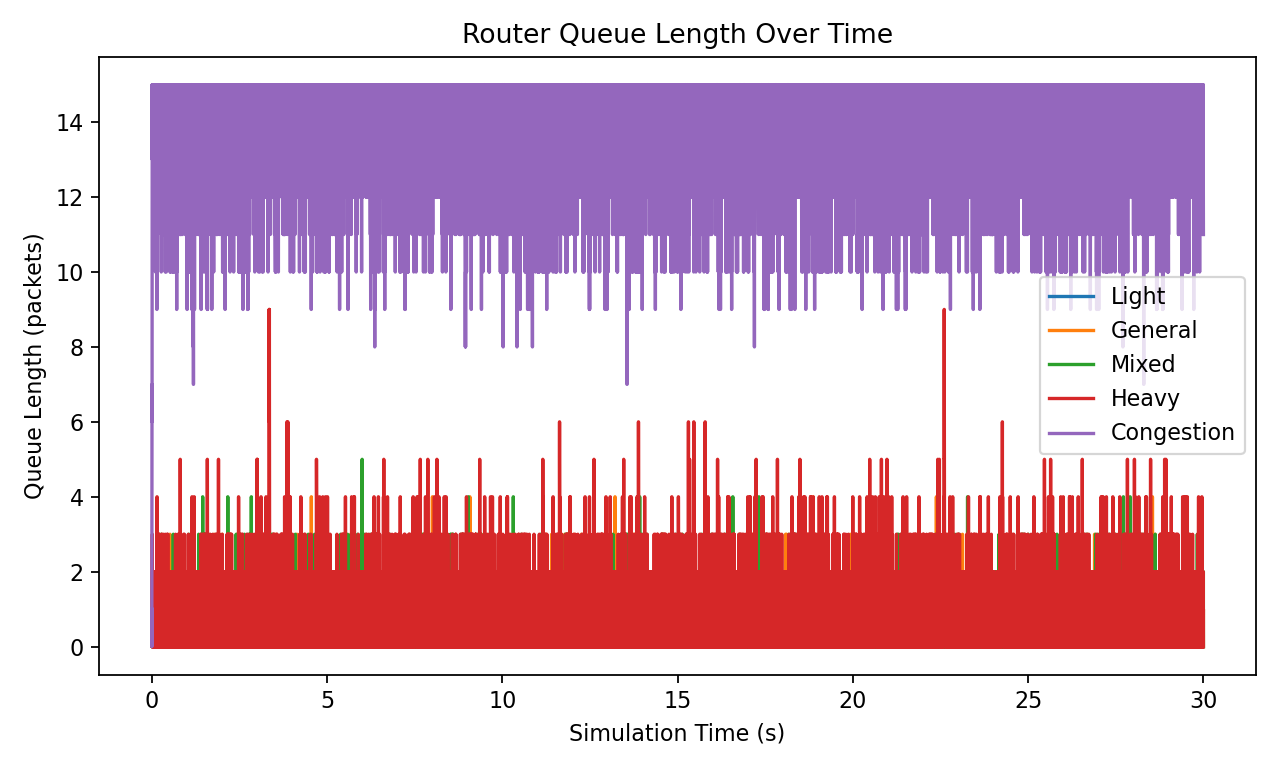
\includegraphics[width=0.9\linewidth]{figures/queue_length_timeseries.png}
  \caption{Queue length over time across scenarios}
\end{figure}

Queue length rises with offered load, peaking in Heavy and Congestion scenarios. Congestion-mode switching limits sustained growth once thresholds are exceeded.

\begin{figure}[h]
  \centering
  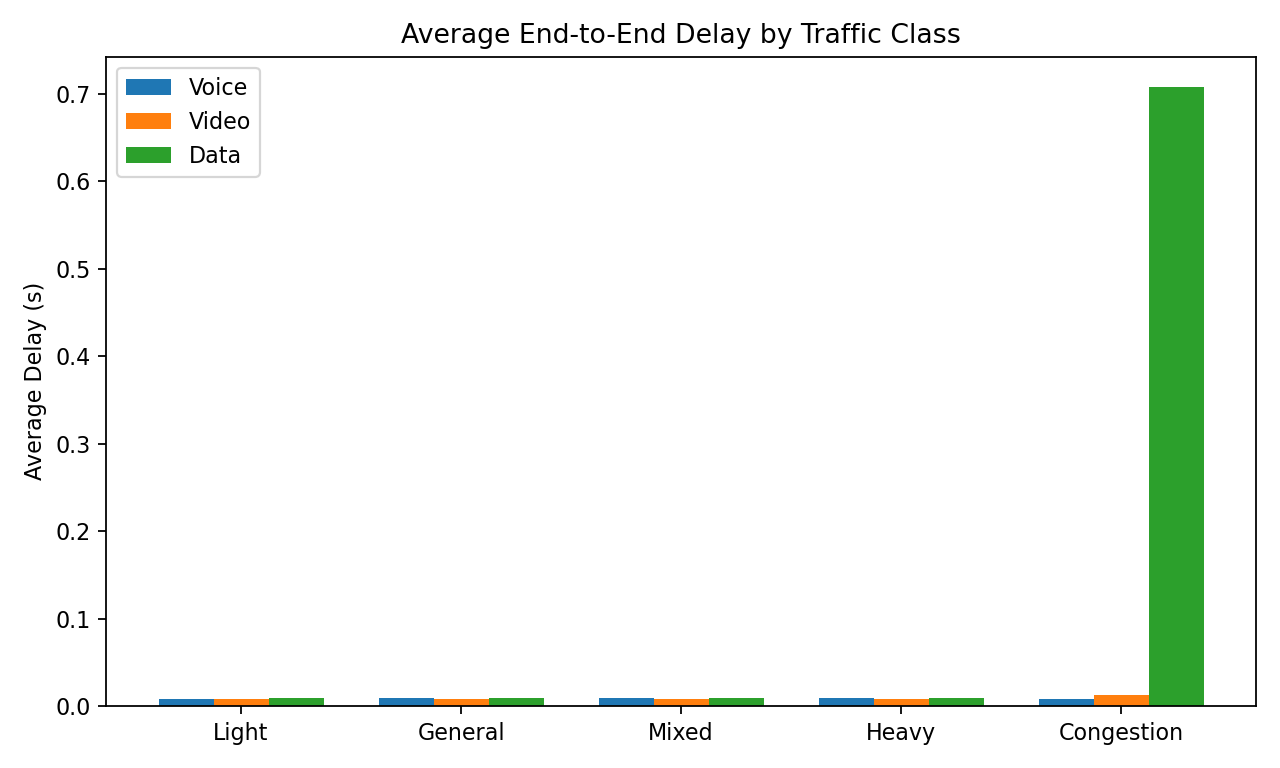
\includegraphics[width=0.9\linewidth]{figures/delay_by_type.png}
  \caption{Average end-to-end delay by traffic class}
\end{figure}

Voice traffic consistently achieves the lowest latency, with video protected relative to data during congestion periods.

\begin{figure}[h]
  \centering
  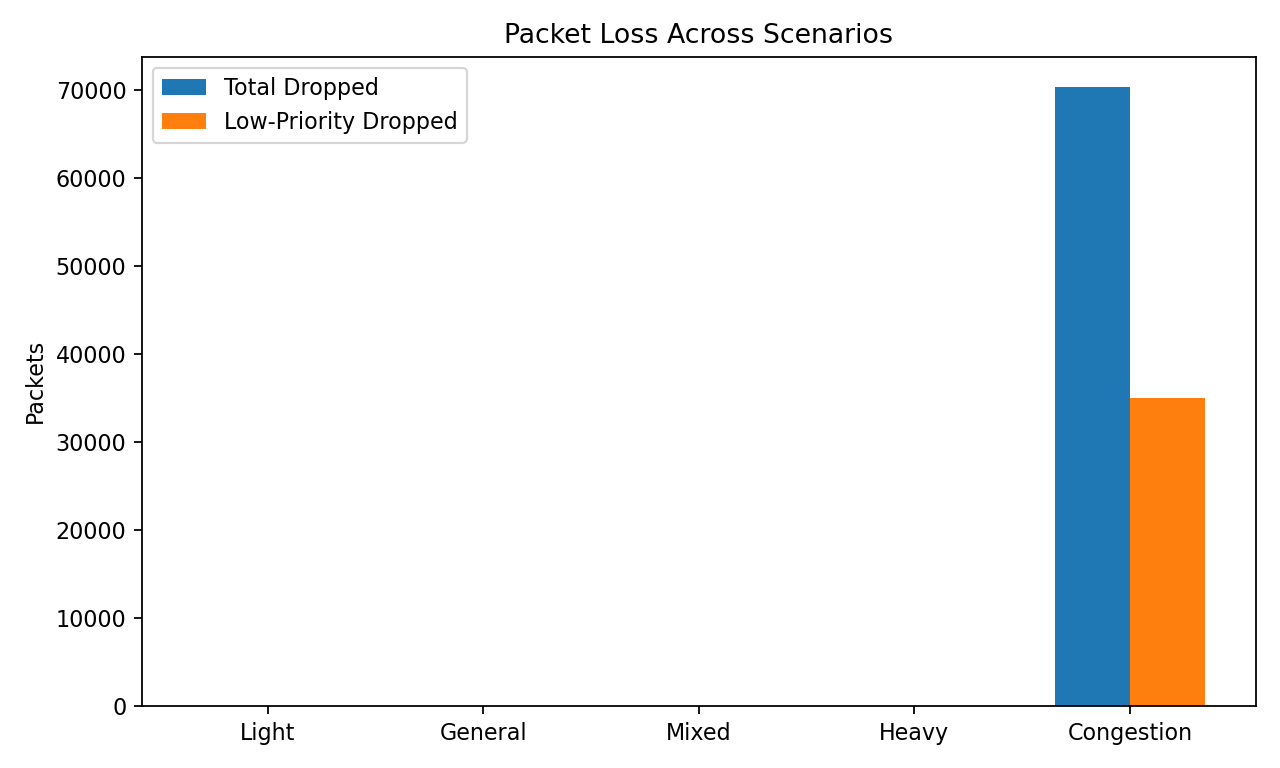
\includegraphics[width=0.9\linewidth]{figures/packet_loss.png}
  \caption{Packet loss across scenarios (total and low-priority)}
\end{figure}

In current runs, if offered load is below service capacity, drops are negligible; otherwise, losses concentrate in the lowest-priority class as intended. The plotting script annotates the chart when all loss values are zero.

\begin{figure}[h]
  \centering
  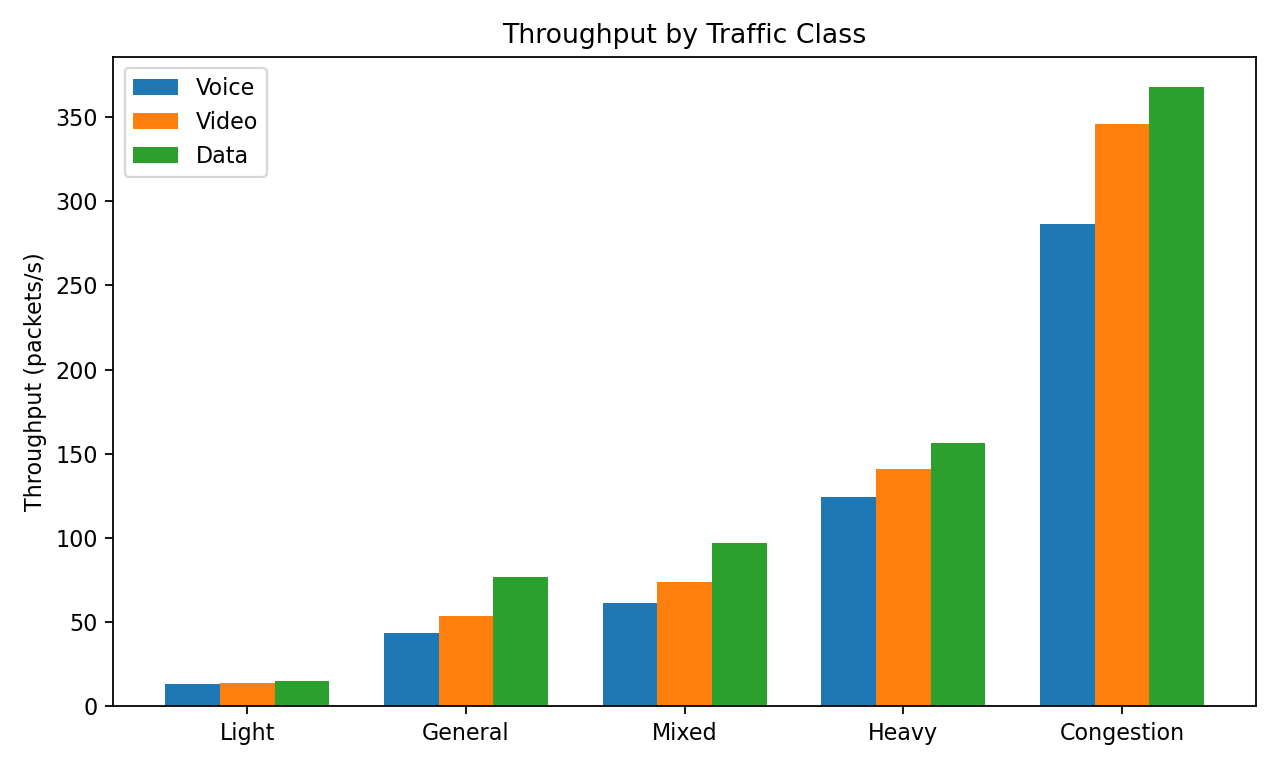
\includegraphics[width=0.9\linewidth]{figures/throughput_by_type.png}
  \caption{Throughput by traffic class across scenarios}
\end{figure}

Throughput for voice and video remains relatively stable, indicating that priority service maintains delivery rates for real-time classes. Data throughput varies more under higher load due to selective dropping in congested mode.

\subsection{Observations}
Key observations include: mode switching aligns with threshold crossings, limiting sustained queue growth; latency protection is strongest for voice while video benefits during peaks; loss behavior depends on offered load relative to the service rate; and results are reproducible via exported scalars and the plotting script.

\section{Discussion}
QoS-AR's adaptive scheduling achieves a practical balance between QoS and resource efficiency. Elevating priority for real-time traffic reduces delay but may increase loss for data during peaks. This trade-off is intentional: latency requirements for voice and video are stricter, while data flows often tolerate retransmissions. The system avoids starvation by returning to normal mode when congestion subsides.

Parameter tuning—specifically, queue capacity, service rate, and thresholds—affects responsiveness. Higher thresholds delay switches but risk larger queues; lower thresholds may switch too often. Careful calibration based on workload is recommended.

\section{Limitations and Threats to Validity}
This study uses a single-router topology, which may not capture multi-hop interactions. The synthetic traffic models approximate real behavior but do not replicate production traces. Service rate versus offered load must be tuned to elicit packet drops; otherwise packet-loss conclusions can be trivial. Results are sensitive to simulation duration and burst configuration, which should be considered when generalizing findings.

\section{Conclusion}
We presented QoS-AR, a minimal, adaptive router that enforces QoS under varied load without heavy dependencies. The design combines priority queuing with congestion-aware mode switching to protect delay-sensitive traffic. Experiments show reduced delays for real-time classes, controlled queue growth, and concentrated packet loss in low-priority traffic under overload. QoS-AR provides a practical approach to QoS enforcement for small-scale deployments and educational settings.

\section{Future Work}
Future directions include multi-router topologies, ML-based congestion prediction, comparison with RED/CoDel, and real-time visualization of router states. Extending the adaptive logic with dynamic thresholding or control-theoretic tuning may further improve responsiveness.

\section*{References}
OMNeT++ User Manual, Version 6.x. Available at \url{https://omnetpp.org/}.

RFC 4594: Configuration Guidelines for DiffServ Service Classes. IETF, 2006.

\appendix
\section{Selected Configuration and Commands}
\noindent Example scenario execution and export:
\begin{verbatim}
./SmartQueue -u Cmdenv -f omnetpp.ini -c Light
./SmartQueue -u Cmdenv -f omnetpp.ini -c Mixed
./SmartQueue -u Cmdenv -f omnetpp.ini -c Heavy
./SmartQueue -u Cmdenv -f omnetpp.ini -c Congestion
opp_scavetool x results/* -o results/scalars.csv -F CSV-R
python3 scripts/plot_metrics.py
\end{verbatim}

\section{Code Snippet: Router Drop Counters}
\begin{lstlisting}[language=C++,caption={Illustrative drop counter update}]
// in AdaptiveRouter::handleIncomingPacket
if (priorityQueue.isFull()) {
    packetsDropped++;
    if (pkt.priority == LOW) lowPriorityDropped++;
    delete pkt; // drop
    return;
}
priorityQueue.enqueue(pkt);
\end{lstlisting}

\end{document}